% Template for PLoS
% Version 1.0 January 2009
%
% To compile to pdf, run:
% latex plos.template
% bibtex plos.template
% latex plos.template
% latex plos.template
% dvipdf plos.template

\documentclass[10pt]{article}

% amsmath package, useful for mathematical formulas
\usepackage{amsmath}
% amssymb package, useful for mathematical symbols
\usepackage{amssymb}

% graphicx package, useful for including eps and pdf graphics
% include graphics with the command \includegraphics
\usepackage{graphicx}

% cite package, to clean up citations in the main text. Do not remove.
\usepackage{cite}

\usepackage{color} 

\usepackage{pdfpages}

% Use doublespacing - comment out for single spacing
%\usepackage{setspace} 
%\doublespacing

% Text layout
\topmargin 0.0cm
\oddsidemargin 0.5cm
\evensidemargin 0.5cm
\textwidth 16cm 
\textheight 21cm

% Bold the 'Figure #' in the caption and separate it with a period
% Captions will be left justified
\usepackage[labelfont=bf,labelsep=period,justification=raggedright]{caption}

% Use the PLoS provided bibtex style
\bibliographystyle{plos2009}

% Remove brackets from numbering in List of References
\makeatletter
\renewcommand{\@biblabel}[1]{\quad#1.}
\makeatother


% Leave date blank
\date{}

\pagestyle{myheadings}
%% ** EDIT HERE **


%% ** EDIT HERE **
%% PLEASE INCLUDE ALL MACROS BELOW

%% END MACROS SECTION

\begin{document}

% Title must be 150 characters or less
\begin{flushleft}
{\Large
\textbf{Analysis of Nasopharyngeal Carcinoma using Exome Sequencing}
}
% Insert Author names, affiliations and corresponding author email.
\\
J. Reese$^{1}$, 
V. Benstead-Hume$^{1}$, 
G. Benstead-Hume$^{1}$,
G. Benstead-Hume$^{1}$,
K. Hodges$^{1}$,
J. Mulvenna$^{2,\ast}$
\\
\bf{1} Genformatic, LLC, 6301 Highland Hills Drive Austin, TX 78731
\\
\bf{2} Infectious Disease and Cancer, Queensland Institute for Medical Research, Brisbane, Australia.
\\
$\ast$ E-mail: jason.mulvenna@qimr.edu.au
\end{flushleft}

% Please keep the abstract between 250 and 300 words
\section*{Abstract}

% Please keep the Author Summary between 150 and 200 words
% Use first person. PLoS ONE authors please skip this step. 
% Author Summary not valid for PLoS ONE submissions.   
\section*{Author Summary}

\section*{Introduction}

% Results and Discussion can be combined.
\section*{Results}

\subsection*{Somatic mutations in NPC samples}
Of the 4,376 somatic mutations, 147 occur at a position with an existing record in COSMIC and 78 of these cause moderate/high impact mutations in a total of 76 genes.

\subsection*{Mutational signatures in NPC somatic mutations}
In these NPC somatic mutations, C->T mutations predominate, with a smaller number of T->C mutations. This seems to correspond to signature 1B from Alexandrov, et al. 2013, which is thought to be caused by spontaneous deamination of 5-methyl-cytosine.

\section*{Discussion}

% You may title this section "Methods" or "Models". 
% "Models" is not a valid title for PLoS ONE authors. However, PLoS ONE
% authors may use "Analysis" 
\section*{Materials and Methods}

\subsection*{Exome sequencing}

DNA was isolated from six samples, from differentiated NPC tumor tissue (samples 04-S-341B and 08-S-6658A), undifferentiated NPC tumor tissue (samples 04-S-6103A and 12-S-432A) or normal, non-cancerous tissue (samples 05-S-5264F and 08-S-6658C). Only two samples (08-S-6658A and 08-S-6658C) were matched tumor/normal samples from the sample individual. Exome DNA was amplified using standard protocol [WHAT EXOME KIT WAS USED?]. DNA was sequenced using Illumina [WHAT MACHINE?], generating 
a total of 38.78 Gbases of sequence data for all six samples. 

\subsection*{Detection of somatic mutations}
Somatic mutations were detected using exome sequencing data for a tumor/normal pair (samples 08-S-6658A and 08-S-6658C, respectively) from a single individual. Sequencing reads were aligned to the human genomes build HG19 (http://hgdownload.cse.ucsc.edu/goldenPath/hg19/bigZips/chromFa.tar.gz) using BWA version 0.7.5a. 
PCR duplicates were removed using Picard [REF], local realignment and quality score recalibration was performed using GATK version 1.0.5974. From these alignments, we detected somatic mutations using three programs (VarScan2, Strelka and SomaticSniper), and these were combined into a high-confidence set of 4,376 somatic mutations using BAYSIC [REF]. 

\subsection*{Detection of variants in unpaired samples}

Lorem ipsum. 

\subsection*{Characterization of likely driver mutations}
To characterize possible driver mutations among the 4,376 somatic mutations, we selected somatic mutations that 1) occurred at positions in the genome with records in COSMIC (online database of previously observed cancer mutations) and 2) caused moderate to high impact mutations in known genes, as detected by SNPEffect [REF]. 

\subsection*{Characterizing mutational signatures of somatic mutations}
We wrote custom software to characterize the mutational signature of the somatic mutations, after Alexandrov, et al., 2013. Briefly, for each somatic mutation, the original and mutated residue as well as the adjacent 5' and 3' residues were recorded, and a histogram of the mutations was generated (Figure 2). 


% Do NOT remove this, even if you are not including acknowledgments
\section*{Acknowledgments}

%\section*{References}
% The bibtex filename
\bibliography{template}

\section*{Figure Legends}

\subsection*{Figure 1}
\begin{figure}[!ht]
\begin{center}
\ifpdf
% \includepdf[pages={1},scale=0.5]{figure1/figure1.pdf}
\includegraphics[width=6in]{figure1/figure1.pdf}
\else
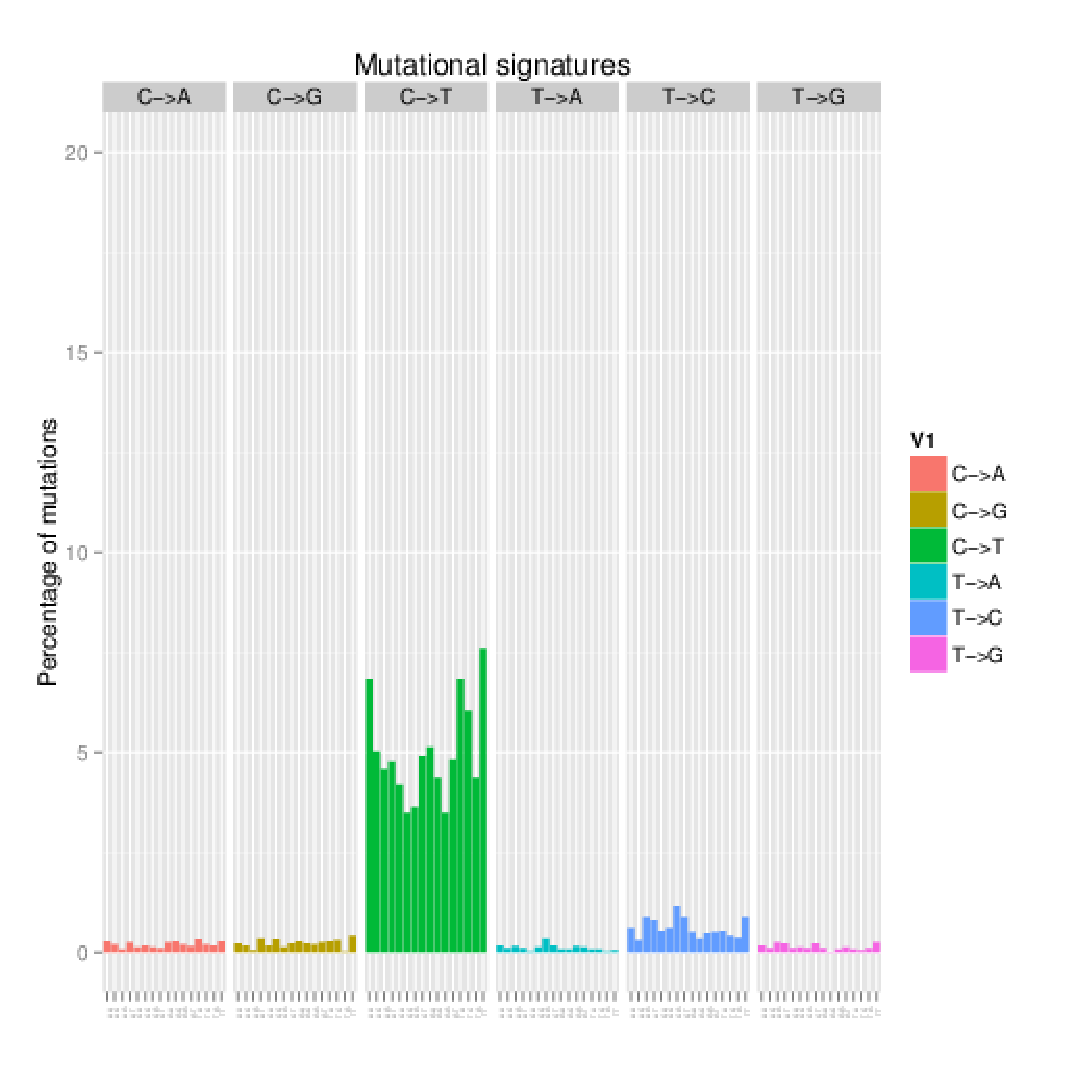
\includegraphics[width=6in]{figure1/mutation_signature.15.30.48_November_05_2013.eps}
\fi
\end{center}
\caption{
{\bf Mutational signature of somatic mutations generated using NPC tumor/normal pair.}  Rest of figure 2  caption.  Caption 
should be left justified, as specified by the options to the caption 
package.
}
\label{Figure_label2}
\end{figure}

\section*{Tables}
\begin{table}[ht] 
\tiny
\caption{Moderate to high-impact somatic mutations with existing COSMIC records} % from /data/experiments/2013_10_combined_NPC_somatic_mutation_calls/cosmic/cosmic_genes.tsv
\centering % used for centering table 
\begin{tabular}{l l} % centered columns (2 columns) 
\hline
Gene symbol & Description \\ [0.5ex] % inserts table 
\hline % inserts single horizontal line 
SPOCD1 & SPOC domain containing 1 \\
EIF2C1 &  \\
IGSF3\_ENST00000369483 &  \\
PRPF3 & PRP3 pre-mRNA processing factor 3 homolog (S. cerevisiae) \\
FLG2 & filaggrin family member 2 \\
SPTA1 & spectrin, alpha, erythrocytic 1 (elliptocytosis 2) \\
OR6N1 & olfactory receptor, family 6, subfamily N, member 1 \\
MR1 & major histocompatibility complex, class I-related \\
CAMSAP1L1 &  \\
USH2A & Usher syndrome 2A (autosomal recessive, mild) \\
USH2A & Usher syndrome 2A (autosomal recessive, mild) \\
ACBD3 & acyl-CoA binding domain containing 3 \\
LYST & lysosomal trafficking regulator \\
RYR2 & ryanodine receptor 2 (cardiac) \\
OR2L13\_ENST00000366478 &  \\
TACR1 & tachykinin receptor 1 \\
KCNJ3 & potassium inwardly-rectifying channel, subfamily J, member... \\
WDSUB1 & WD repeat, sterile alpha motif and U-box domain containing.. \\
TNIK\_ENST00000436636 &  \\
UGT2B28 & UDP glucuronosyltransferase 2 family, polypeptide B28 \\
NR3C2 & nuclear receptor subfamily 3, group C, member 2 \\
DCHS2 & dachsous 2 (Drosophila) \\
GPR98 & G protein-coupled receptor 98 \\
UBLCP1 & ubiquitin-like domain containing CTD phosphatase 1 \\
CASP8AP2 & caspase 8 associated protein 2 \\
PRDM13 & PR domain containing 13 \\
KIAA1244\_ENST00000251691 &  \\
FNDC1 & fibronectin type III domain containing 1 \\
EIF2AK1 & eukaryotic translation initiation factor 2-alpha kinase... \\
CALN1 & calneuron 1 \\
NSUN5\_ENST00000438747 &  \\
GRM8 & glutamate receptor, metabotropic 8 \\
KEL & Kell blood group, metallo-endopeptidase \\
MBOAT4\_ENST00000320542 &  \\
ZFHX4 & zinc finger homeobox 4 \\
FRMPD1 & FERM and PDZ domain containing 1 \\
C9orf156 & chromosome 9 open reading frame 156 \\
COL5A1 & collagen, type V, alpha 1 \\
GPRIN2 & G protein regulated inducer of neurite outgrowth 2 \\
AGAP6 & ArfGAP with GTPase domain, ankyrin repeat and PH domain... \\
ANK3 & ankyrin 3, node of Ranvier (ankyrin G) \\
COL17A1 & collagen, type XVII, alpha 1 \\
GFRA1 & GDNF family receptor alpha 1 \\
CSTF3 & cleavage stimulation factor, 3' pre-RNA, subunit 3, 77kDa \\
OR4X1 & olfactory receptor, family 4, subfamily X, member 1 \\
OR4C3 & olfactory receptor, family 4, subfamily C, member 3 \\
OR5T2 & olfactory receptor, family 5, subfamily T, member 2 \\
OR5B17 & olfactory receptor, family 5, subfamily B, member 17 \\
EHD1 & EH-domain containing 1 \\
KRTAP5-8 & keratin associated protein 5-8 \\
KIAA1377 & KIAA1377 \\
GRIA4 & glutamate receptor, ionotropic, AMPA 4 \\
CUL5 & cullin 5 \\
OR10G9 & olfactory receptor, family 10, subfamily G, member 9 \\
CD163L1 & CD163 molecule-like 1 \\
CLIP1 & CAP-GLY domain containing linker protein 1 \\
ATP12A & ATPase, H+/K+ transporting, nongastric, alpha polypeptide \\
KIAA0564 &  \\
COL4A2 & collagen, type IV, alpha 2 \\
AHNAK2\_ENST00000333244 &  \\
ANKRD11 & ankyrin repeat domain 11 \\
TNFRSF11A & tumor necrosis factor receptor superfamily, member 11a \\
CD226 & CD226 molecule \\
PLIN4\_ENST00000301286 &  \\
ZNF626\_ENST00000392298 &  \\
ZNF229 & zinc finger protein 229 \\
SIGLEC12 & sialic acid binding Ig-like lectin 12 (gene/pseudogene) \\
SIGLEC12 & sialic acid binding Ig-like lectin 12 (gene/pseudogene) \\
ZNF808 & zinc finger protein 808 \\
SLC27A5 & solute carrier family 27 (fatty acid transporter) \\
TP53TG5 & TP53 target 5 \\
PREX1 & phosphatidylinositol-3,4,5-trisphosphate-dependent Rac exchange \\
PCNT & pericentrin \\
RAB36 & RAB36, member RAS oncogene family \\
ENTHD1 & ENTH domain containing 1 \\
PARVB & parvin, beta \\
USP9X\_ENST00000324545 &  \\
PHKA1 & phosphorylase kinase, alpha 1 (muscle) \\
\hline %inserts single line 
\end{tabular} 
\label{table:nonlin} % is used to refer this table in the text 
\end{table} 

\end{document}

